%-------------------------------------------------------------------
% bachelor thesis
%
% topic: ACDC4JS - How to analyze a JavaScript garbage collector
%
% create by: Mario Preishuber
% create date: 2014, Jan 01.
%-------------------------------------------------------------------

\chapter{ACDC4JS}

\section{Preparation}
	For developing a tool like ACDC4JS it is necessary to get some information before starting with implementing. The Figure \ref{fig:heap_structure_analysis} on page \pageref{fig:heap_structure_analysis} shows the toolchain used to analysis the structure of real JavaScript applications. For the simulation of realistic user interaction on an web page the tool called \texttt{AutomatedUserInteraction} (see section \ref{sec:automated_user_interaction}) is used in combination with a custom version of Chromium. The custom Chromium version produces periodic a snapshot of the heap (for details see section \ref{sec:custom_chromium}). These snapshots are analyzed by the so-called \texttt{HeapSnapshotAnalyzer} (see section \ref{sec:heap_snapshot_analyzer}). The \texttt{HeapSnapshotAnalyzer} used for the analysis an PostgreSQL database in version 9.3 \cite{Psql13}.

	\begin{figure}
		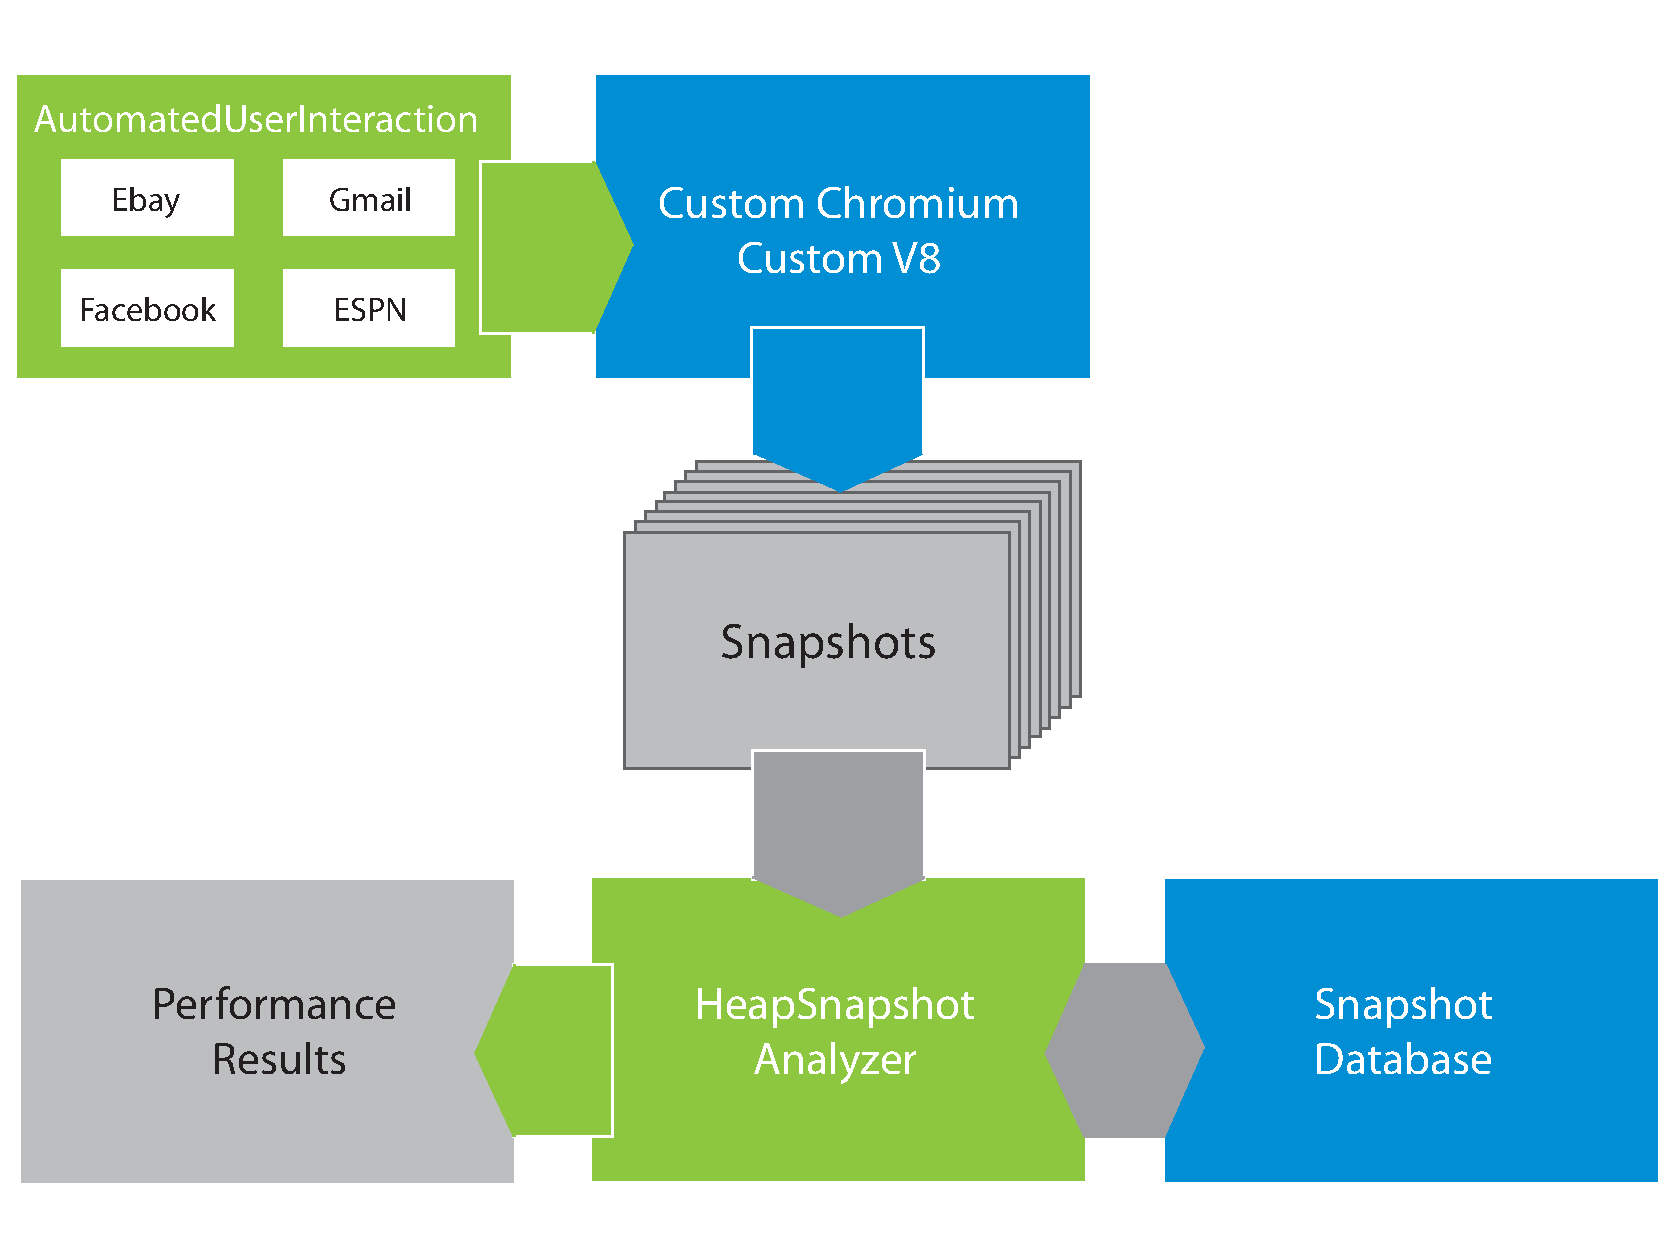
\includegraphics[width=0.7\textwidth]{solution_h.pdf}
		\caption{Tool chain to analyze the JavaScript heap structure of a real web application}
		\label{fig:heap_structure_analysis}
	\end{figure}

	\subsection{AutomatedUserInteraction} \label{sec:automated_user_interaction}
		We want to analyze the heap structure of real web applications. So two things are important, one thing is to automate the interaction on the web page and the other is to enable an easy repeat of the interaction. This leads us to the use of SeleniumHQ\cite{Sele13}. SeleniumHQ is a framework for browser automation. 

		\

		The \texttt{AutomatedUserInteraction} is an Java application which uses SeleniumHQ. This tool contains all automated interaction for all web pages we to analyze. The table \ref{tab:user_interactions} below shows all anaylzed web pages. To execute some interaction on a web page we used our own custom binary of Chromium (for details see section \ref{sec:custom_chromium} on page \pageref{sec:custom
		_chromium}).

		\begin{table}
			\centering
			\begin{tabular}{|c||l|}
				\hline
				\textbf{type} 	& \textbf{web pages}		\\ \hline \hline
				\textbf{news} 	& cnn\cite{Cnn13}, the economist\cite{Econ13}, espn	\\ \hline
				\textbf{mail} 	& hotmail, gmail 			\\ \hline
				\textbf{search}	& bing, google				\\ \hline
				\textbf{social}	& facebook, google+			\\ \hline
				\textbf{maps}	& bing, google				\\ \hline
				\textbf{shop}	& amazon, ebay				\\ \hline
			\end{tabular}
			\caption{Anaylzed real web pages}
			\label{tab:user_interactions}
		\end{table}
	\subsection{Custom Chromium} \label{sec:custom_chromium}
		

	\subsection{HeapSnapshotAnalyzer} \label{sec:heap_snapshot_analyzer}

